\documentclass[a4paper]{article}
\usepackage[utf8]{inputenc}
\usepackage{fancyhdr}
\usepackage{geometry}
\usepackage{listings}
\usepackage{graphicx}
\usepackage{algorithmic}
\usepackage{float}
\usepackage{hyperref}

\lstset{
    language=Python,
    breaklines=true,
    numbers=left,
    frame=lines
}

\pagestyle{fancyplain}

\title{User Manual}
\author{Harry Milne}
\date{March 2014}

\lhead{Harry Milne}
\chead{Candidate Number: 2677}
\rhead{Centre Number: 22169}

\begin{document}
\maketitle
\tableofcontents
\newpage

\section{Introduction}

The intended audience of this system is a 
\section{Installation}
\subsection{Prerequisite Installation}

\subsection{System Installation}
If you do not already have the files they are available for download at: \url{https://github.com/harrymilne/face_recognition_a2}.
This repository has two root folders, `code' and `docs', Python files for the running of the client and server are under code.
Once you are in the code directory this then has 3 folders, `client', `db\_browser' and `server', the `server' and `db\_browser'
folders need to be on the same computer, whereas the client needs to be placed on a computer with access to a network capable of
connecting to the computer which has the `server' and `db\_browser' folders on. 

\subsubsection{Client}
The client software must be installed anywhere you want end-users to be able to control the system, the code can be ran on a 
raspberry pi or on a `normal computer'. 
The client (face recognition) requires a Python package called SimpleCV, to install this you must first 
download the `superpack' from simplecv.org/download (shown in figure~\ref{fig:simplecv}).  This installs all of the dependencies you need for the client program.

\begin{figure}[H]
    \label{fig:simplecv}
    \centering
    \caption{A screenshot of the SimpleCV website where it is possible to download the `superpack'.}
    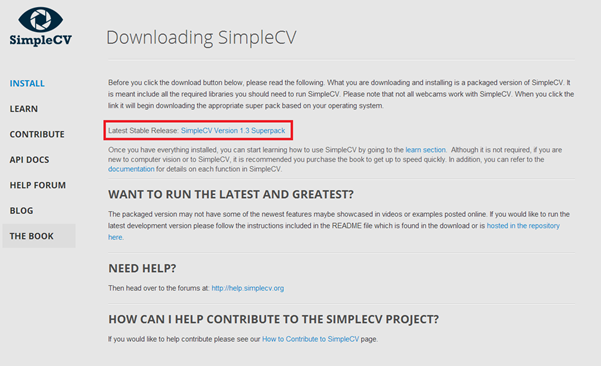
\includegraphics[scale=0.7]{../shared_assets/screenshots/manual/simplecv_download.png}
\end{figure}

The files included with the downloaded repository will include an example configuration file called `client.cfg'. As shown
below in figure~\ref{fig:clientcfg}, this must but set to use values that suite your system needs. To find the `haar\_cascade'
path you must find where your Python installation resides and check `dist-packages' for the `SimpleCV' folder, then it should
be under `Features/HaarCascades' as of version 1.3.

\begin{figure}[H]
    \label{fig:clientcfg}
    \centering
    \caption{Example client configuration included in code repository.}
    \lstinputlisting{../../code/client/client.cfg}
\end{figure}



After downloading and installing the relevant `superpack' for your system, you can run the client with Python version 2.7.

\subsection{Server}
The serv

\section{Tutorial}
    \subsection{Introduction}
    \subsection{Assumptions}
    \subsection{FAQ}
    \subsection{FAQ}
    \subsection{FAQ}
\section{Errors}
    \subsection{SimpleCV/Camera related}
    \subsection{Network related}
    \subsection{Settings}
\section{System Recovery}
    \subsection{Backing up data}
    \subsection{Restoring data}

\end{document}
